\documentclass[13pt,a4paper,oneside]{article}
\usepackage[ngerman]{babel}
\usepackage[utf8]{inputenc}
\usepackage{amsmath}
\usepackage{amsfonts}
\usepackage{amssymb}
\usepackage{graphicx}
\usepackage[left=2cm,right=2cm,top=2cm,bottom=2cm]{geometry}
\usepackage{fancyhdr}
\usepackage{graphicx}
\usepackage{listings}
\usepackage{xcolor}
\usepackage{color, colortbl}
\definecolor{codegreen}{rgb}{0,0.6,0}
\definecolor{codegray}{rgb}{0.5,0.5,0.5}
\definecolor{codepurple}{rgb}{0.58,0,0.82}
\definecolor{backcolour}{rgb}{0.95,0.95,0.92}
\definecolor{codeLightCyan}{rgb}{0.88,1,1}
\definecolor{codered}{rgb}{255,193,193}

%Includes "References" in the table of contents
\usepackage[nottoc]{tocbibind}

\lstdefinestyle{mystyle}{
    backgroundcolor=\color{backcolour},   
    commentstyle=\color{codegreen},
    keywordstyle=\color{magenta},
    numberstyle=\tiny\color{codegray},
    stringstyle=\color{codepurple},
    basicstyle=\ttfamily\footnotesize,
    breakatwhitespace=false,         
    breaklines=true,                 
    captionpos=b,                    
    keepspaces=true,                 
    numbers=left,                    
    numbersep=5pt,                  
    showspaces=false,                
    showstringspaces=false,
    showtabs=false,                  
    tabsize=2
}

\lstset{style=mystyle}
%\usepackage{float}
%\usepackage{wrapfig}
\usepackage{float}
\restylefloat{table}
%link
\usepackage{hyperref}
\author{Vantinh}
\title{ICW}
\date{\today}

\pagestyle{fancy}
\fancyhf{}
\lhead{Independent Coursework (ICW 1)- Master Angewandte Informatik-HTW Berlin-SS2020}
\rfoot{Seite \thepage}

\begin{document}
\begin{center}
{\Huge Dichte-basierte Clusteringverfahren für große Datenmengen Teil B}\\
Van Tinh Chu
\textit{HTW Berlin}\\
Berlin, Germany\\
s01567851@htw-berlin.de
\end{center}

\tableofcontents% Inhaltsverzeichnis
\listoffigures% Abbildungsverzeichnis
\listoftables% Tabellenverzeichnis

\newpage
\paragraph{Abstrakt}
Aus Teil  A von Independent  Course haben wir schon drei Algorithmen(DBSCAN, HDBSCAN, OPTICS) probiert, um den besten Algorithmus finden zu können. Im Rahmen des Projekts erweitern wir weiterhin im drei Monat, um nach dem Ersatz der oben Algorithmus zu suchen, nämlich ein paar Algorithmen in diesem Bericht erforscht werden. Dabei werden das Verfahren und die  Komplexität von Algorithmen auch geforscht, damit ein guter Überblick für die Forschung ausgeworfen wird. Dann wird ein Datensatz in 100 bis 200 Dimension mit 2 bis 5 Millionen Datenmenge geschaffen und untersucht, damit ein Algorithmus mit diesen Datenmenge innerhalb 5 Tage laufen kann.
\paragraph{Keywords:} Clustering, density-based clustering, hierarchical clustering, dichbasierte Clustering,High dimension multiview data OptimizationSpark
\section{Einleitung}
Clustering spielt eine wichtige Rolle in dem Bereich Machine Learning. Mit Hilfe der machenden Cluserting werden Datenmenge in der getrennt Klasse sortiert. Aus diese Analyse wird die wichtige Information ausgezogen. Im IT Bereich gibt es mehre Algorithmen , um die Datenmenge zu klassifizieren. Trotzdem sollte ein suchender Algorithmus gefunden werden, damit das Problem der großen Datenmenge innerhalb 5 Tage gelöst werden, damit die Cluster im dieser  Datenmenge entdeckt werden kann.
\section{eine Umfrage der Clustering für große Datenmenge}
Im Internet gab es schon ein paar Berichte über die Verarbeitung der  Clusteringsprozess. Es ist jedoch unklare Ergebnisse für die riesig  Datenmenge in der höhe Dimension. Deswegen sollte es klar sein,welcher Algorithmus besser verwendet werden sollte. Durch den Bericht \cite{6832486} können wir erkennen, dass die Ergebnisse der Algorithmen in einer Tabelle eingefügt werden.
\paragraph{Clustering - Algorithment - Kategorien}
Damit die Verwirrung von Clustering-Kategorien vermieden werden kann, muss eine Überblick der Cluster ausgegeben werden, weil es nun viele Algorithmen für Clustering gibt. Zudem werden das Verfahren und Verarbeitung von jedem Algorithmus unter zusammengefasst. 
\\Abbildung \ref{fig:image_categories}
    \begin{figure}[!h]
        \centering
        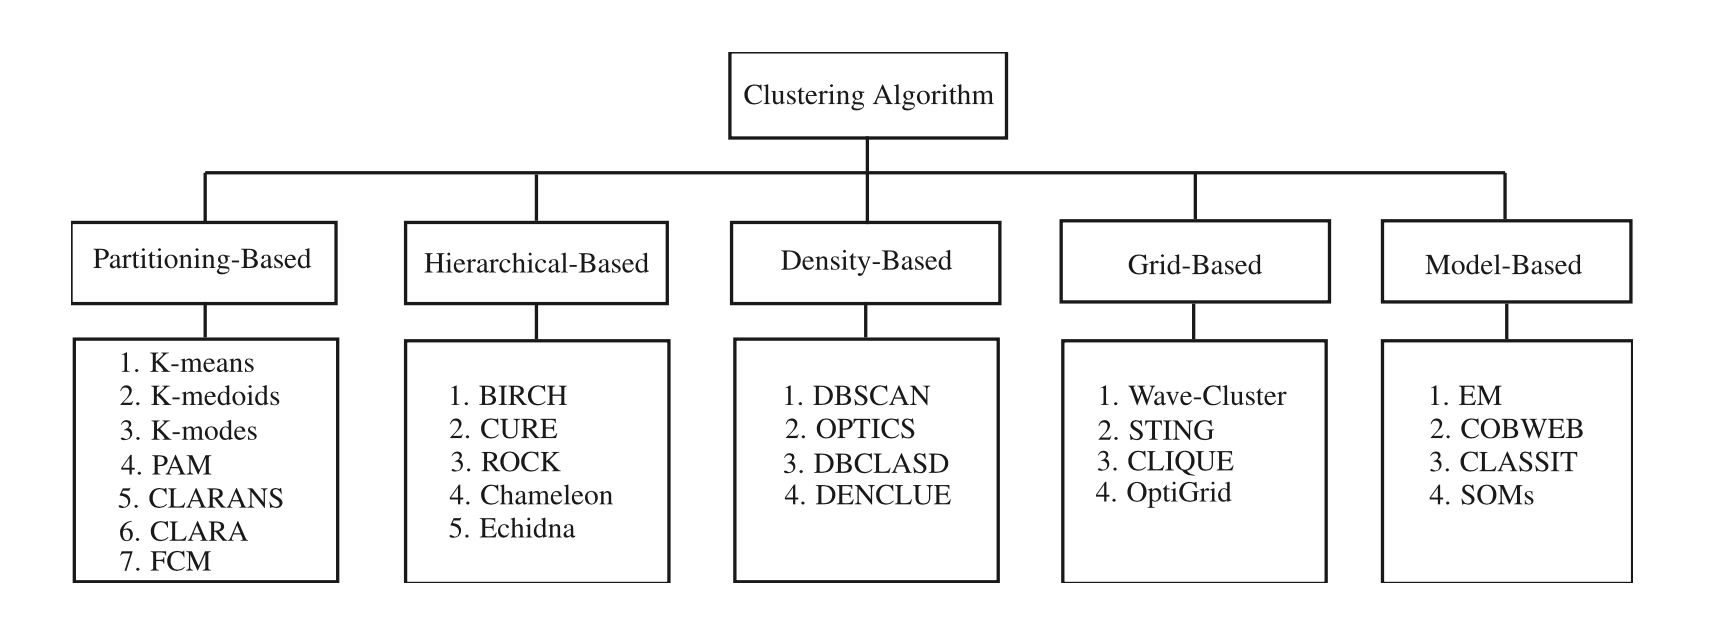
\includegraphics[width=\textwidth]{images/categories.png}
        \caption[Eine Taxonomie von wichtigen Clus- teralgorithmen]{Eine Taxonomie von wichtigen Clus- teralgorithmen}
        \label{fig:image_categories}
    \end{figure}
\\
\begin{list}{•}
\item \textbf{Partitioning-based:} 
\item \textbf{Hierarchical-ased:} 
\item \textbf{Density-based:} 
\item \textbf{Grid-based:} 
\item \textbf{Model-based:} 
\end{list}
\cite{6832486}
\section{5 häufigste Algorithmen für Clustering in Machine Learning}
Es gab zurzeit verschiedene Algorithmen für den Process des Clustering
\footnote{\href{https://towardsdatascience.com/the-5-clustering-algorithms-data-scientists-need-to-know-a36d136ef68}https://towardsdatascience.com/the-5-clustering-algorithms-data-scientists-need-to-know-a36d136ef68}

\section{K-Means Clustering}
O(n) komplexitat
k means ist noch langer als minibatch kmeans
https://scikit$\-$learn.org/stable/modules/generated/

%sklearn.cluster.KMeans.html#sklearn.cluster.KMeans%
\section{Minibatch kmean}
%https://scikit-learn.org/stable/modules/generated/sklearn.cluster.MiniBatchKMeans.html#sklearn.cluster.MiniBatchKMeans%

fragen auf stack over flow
https://stackoverflow.com/questions/47270604/python-kmeans-clustering-for-large-datasets

he so la : 
$kmeans = MiniBatchKMeans(n_clusters=100,
random_state = 0,
batch_size = 300,
max_iter = 100).fit(X)
3 trrieu = 79s
1 trieu = 22s	
4 trieu = 116.7942 s 
(5000000, 100) 5 trieu 
Elapsed time to cluster in MInibatch kmeans :  190.0804 s 
$
\section{ALl Sklearn}
all clustering aus clutstering
https://github.com/scikit-learn/scikit-learn/tree/0fb307bf39bbdacd6ed713c00724f8f871d60370/sklearn/cluster
\section{FUZZY-CMEANS (FCM) und EM	}
%example: https://www.youtube.com/watch?v=FA$\-$hJBu5Bkc&ab$\_$channel=TheAcademicia%
$https://github.com/scikit-fuzzy/scikit-fuzzy$
\section{OptiGrid}
Beispiel: Optigrid
https://github.com/mexxexx/Optigrid/blob/master/optigrid.py
\section{B. BIRCH}
not good
\section{C. DENCLUE}
not gut ,1000 du lieu ma da bi die, va cai thang kia no tu viet chu ko phai cua bon sklearn
\section{EXPECTATION-MAXIMIZATION (EM)}


\section{Zusammenfassung}

\newpage
%Sets the bibliography style to UNSRT and imports the 
%bibliography file "samples.bib".
\bibliographystyle{unsrt}
\bibliography{sample}

\end{document} 
